\documentclass[twoside]{book}

% Packages required by doxygen
\usepackage{calc}
\usepackage{doxygen}
\usepackage{graphicx}
\usepackage[utf8]{inputenc}
\usepackage{makeidx}
\usepackage{multicol}
\usepackage{multirow}
\usepackage{fixltx2e}
\PassOptionsToPackage{warn}{textcomp}
\usepackage{textcomp}
\usepackage[nointegrals]{wasysym}
\usepackage[table]{xcolor}

% Font selection
\usepackage[T1]{fontenc}
\usepackage{mathptmx}
\usepackage[scaled=.90]{helvet}
\usepackage{courier}
\usepackage{amssymb}
\usepackage{sectsty}
\renewcommand{\familydefault}{\sfdefault}
\allsectionsfont{%
  \fontseries{bc}\selectfont%
  \color{darkgray}%
}
\renewcommand{\DoxyLabelFont}{%
  \fontseries{bc}\selectfont%
  \color{darkgray}%
}
\newcommand{\+}{\discretionary{\mbox{\scriptsize$\hookleftarrow$}}{}{}}

% Page & text layout
\usepackage{geometry}
\geometry{%
  a4paper,%
  top=2.5cm,%
  bottom=2.5cm,%
  left=2.5cm,%
  right=2.5cm%
}
\tolerance=750
\hfuzz=15pt
\hbadness=750
\setlength{\emergencystretch}{15pt}
\setlength{\parindent}{0cm}
\setlength{\parskip}{0.2cm}
\makeatletter
\renewcommand{\paragraph}{%
  \@startsection{paragraph}{4}{0ex}{-1.0ex}{1.0ex}{%
    \normalfont\normalsize\bfseries\SS@parafont%
  }%
}
\renewcommand{\subparagraph}{%
  \@startsection{subparagraph}{5}{0ex}{-1.0ex}{1.0ex}{%
    \normalfont\normalsize\bfseries\SS@subparafont%
  }%
}
\makeatother

% Headers & footers
\usepackage{fancyhdr}
\pagestyle{fancyplain}
\fancyhead[LE]{\fancyplain{}{\bfseries\thepage}}
\fancyhead[CE]{\fancyplain{}{}}
\fancyhead[RE]{\fancyplain{}{\bfseries\leftmark}}
\fancyhead[LO]{\fancyplain{}{\bfseries\rightmark}}
\fancyhead[CO]{\fancyplain{}{}}
\fancyhead[RO]{\fancyplain{}{\bfseries\thepage}}
\fancyfoot[LE]{\fancyplain{}{}}
\fancyfoot[CE]{\fancyplain{}{}}
\fancyfoot[RE]{\fancyplain{}{\bfseries\scriptsize Generated on Fri Jun 27 2014 13\+:50\+:53 for U\+N\+I\+X daemon for U\+D\+P communication by Doxygen }}
\fancyfoot[LO]{\fancyplain{}{\bfseries\scriptsize Generated on Fri Jun 27 2014 13\+:50\+:53 for U\+N\+I\+X daemon for U\+D\+P communication by Doxygen }}
\fancyfoot[CO]{\fancyplain{}{}}
\fancyfoot[RO]{\fancyplain{}{}}
\renewcommand{\footrulewidth}{0.4pt}
\renewcommand{\chaptermark}[1]{%
  \markboth{#1}{}%
}
\renewcommand{\sectionmark}[1]{%
  \markright{\thesection\ #1}%
}

% Indices & bibliography
\usepackage{natbib}
\usepackage[titles]{tocloft}
\setcounter{tocdepth}{3}
\setcounter{secnumdepth}{5}
\makeindex

% Hyperlinks (required, but should be loaded last)
\usepackage{ifpdf}
\ifpdf
  \usepackage[pdftex,pagebackref=true]{hyperref}
\else
  \usepackage[ps2pdf,pagebackref=true]{hyperref}
\fi
\hypersetup{%
  colorlinks=true,%
  linkcolor=blue,%
  citecolor=blue,%
  unicode%
}

% Custom commands
\newcommand{\clearemptydoublepage}{%
  \newpage{\pagestyle{empty}\cleardoublepage}%
}


%===== C O N T E N T S =====

\begin{document}

% Titlepage & ToC
\hypersetup{pageanchor=false,
             bookmarks=true,
             bookmarksnumbered=true,
             pdfencoding=unicode
            }
\pagenumbering{roman}
\begin{titlepage}
\vspace*{7cm}
\begin{center}%
{\Large U\+N\+I\+X daemon for U\+D\+P communication \\[1ex]\large v1.\+0 }\\
\vspace*{1cm}
{\large Generated by Doxygen 1.8.7}\\
\vspace*{0.5cm}
{\small Fri Jun 27 2014 13:50:53}\\
\end{center}
\end{titlepage}
\clearemptydoublepage
\tableofcontents
\clearemptydoublepage
\pagenumbering{arabic}
\hypersetup{pageanchor=true}

%--- Begin generated contents ---
\chapter{Todo List}
\label{todo}
\hypertarget{todo}{}

\begin{DoxyRefList}
\item[\label{todo__todo000002}%
\hypertarget{todo__todo000002}{}%
File \hyperlink{atmega16_8h}{atmega16.h} ]none  
\item[\label{todo__todo000017}%
\hypertarget{todo__todo000017}{}%
File \hyperlink{buffer_8c}{buffer.c} ]none  
\item[\label{todo__todo000018}%
\hypertarget{todo__todo000018}{}%
File \hyperlink{buffer_8h}{buffer.h} ]none  
\item[\label{todo__todo000015}%
\hypertarget{todo__todo000015}{}%
File \hyperlink{common_8h}{common.h} ]none  
\item[\label{todo__todo000004}%
\hypertarget{todo__todo000004}{}%
File \hyperlink{enc28j60_8c}{enc28j60.c} ]none  
\item[\label{todo__todo000003}%
\hypertarget{todo__todo000003}{}%
File \hyperlink{enc28j60_8h}{enc28j60.h} ]none  
\item[\label{todo__todo000001}%
\hypertarget{todo__todo000001}{}%
File \hyperlink{freq_8h}{freq.h} ]none  
\item[\label{todo__todo000005}%
\hypertarget{todo__todo000005}{}%
File \hyperlink{icp_8c}{icp.c} ]none  
\item[\label{todo__todo000006}%
\hypertarget{todo__todo000006}{}%
File \hyperlink{icp_8h}{icp.h} ]none  
\item[\label{todo__todo000007}%
\hypertarget{todo__todo000007}{}%
File \hyperlink{leds_8c}{leds.c} ]none  
\item[\label{todo__todo000008}%
\hypertarget{todo__todo000008}{}%
File \hyperlink{leds_8h}{leds.h} ]none  
\item[\label{todo__todo000019}%
\hypertarget{todo__todo000019}{}%
File \hyperlink{main_8c}{main.c} ]none  
\item[\label{todo__todo000009}%
\hypertarget{todo__todo000009}{}%
File \hyperlink{net_8c}{net.c} ]none  
\item[\label{todo__todo000010}%
\hypertarget{todo__todo000010}{}%
File \hyperlink{net_8h}{net.h} ]none  
\item[\label{todo__todo000011}%
\hypertarget{todo__todo000011}{}%
File \hyperlink{spi_8c}{spi.c} ]none  
\item[\label{todo__todo000012}%
\hypertarget{todo__todo000012}{}%
File \hyperlink{spi_8h}{spi.h} ]none  
\item[\label{todo__todo000016}%
\hypertarget{todo__todo000016}{}%
File \hyperlink{stdbool_8h}{stdbool.h} ]none  
\item[\label{todo__todo000013}%
\hypertarget{todo__todo000013}{}%
File \hyperlink{timer0_8c}{timer0.c} ]none  
\item[\label{todo__todo000014}%
\hypertarget{todo__todo000014}{}%
File \hyperlink{timer0_8h}{timer0.h} ]none 
\end{DoxyRefList}
\chapter{Bug List}
\label{bug}
\hypertarget{bug}{}

\begin{DoxyRefList}
\item[\label{bug__bug000002}%
\hypertarget{bug__bug000002}{}%
File \hyperlink{atmega16_8h}{atmega16.h} ]none  
\item[\label{bug__bug000017}%
\hypertarget{bug__bug000017}{}%
File \hyperlink{buffer_8c}{buffer.c} ]none  
\item[\label{bug__bug000018}%
\hypertarget{bug__bug000018}{}%
File \hyperlink{buffer_8h}{buffer.h} ]none  
\item[\label{bug__bug000015}%
\hypertarget{bug__bug000015}{}%
File \hyperlink{common_8h}{common.h} ]none  
\item[\label{bug__bug000004}%
\hypertarget{bug__bug000004}{}%
File \hyperlink{enc28j60_8c}{enc28j60.c} ]'enc\+\_\+send\+\_\+packet' gives a warning with compiler option '-\/\+Woverflow'. You can devide as bytes the 16-\/bit registers.  
\item[\label{bug__bug000003}%
\hypertarget{bug__bug000003}{}%
File \hyperlink{enc28j60_8h}{enc28j60.h} ]none  
\item[\label{bug__bug000001}%
\hypertarget{bug__bug000001}{}%
File \hyperlink{freq_8h}{freq.h} ]none  
\item[\label{bug__bug000005}%
\hypertarget{bug__bug000005}{}%
File \hyperlink{icp_8c}{icp.c} ]none  
\item[\label{bug__bug000006}%
\hypertarget{bug__bug000006}{}%
File \hyperlink{icp_8h}{icp.h} ]none  
\item[\label{bug__bug000007}%
\hypertarget{bug__bug000007}{}%
File \hyperlink{leds_8c}{leds.c} ]none  
\item[\label{bug__bug000008}%
\hypertarget{bug__bug000008}{}%
File \hyperlink{leds_8h}{leds.h} ]none  
\item[\label{bug__bug000019}%
\hypertarget{bug__bug000019}{}%
File \hyperlink{main_8c}{main.c} ]51. signal has not readed!  
\item[\label{bug__bug000009}%
\hypertarget{bug__bug000009}{}%
File \hyperlink{net_8c}{net.c} ]none  
\item[\label{bug__bug000010}%
\hypertarget{bug__bug000010}{}%
File \hyperlink{net_8h}{net.h} ]none  
\item[\label{bug__bug000011}%
\hypertarget{bug__bug000011}{}%
File \hyperlink{spi_8c}{spi.c} ]none  
\item[\label{bug__bug000012}%
\hypertarget{bug__bug000012}{}%
File \hyperlink{spi_8h}{spi.h} ]none  
\item[\label{bug__bug000016}%
\hypertarget{bug__bug000016}{}%
File \hyperlink{stdbool_8h}{stdbool.h} ]none  
\item[\label{bug__bug000013}%
\hypertarget{bug__bug000013}{}%
File \hyperlink{timer0_8c}{timer0.c} ]none  
\item[\label{bug__bug000014}%
\hypertarget{bug__bug000014}{}%
File \hyperlink{timer0_8h}{timer0.h} ]none 
\end{DoxyRefList}
\chapter{File Index}
\section{File List}
Here is a list of all files with brief descriptions\+:\begin{DoxyCompactList}
\item\contentsline{section}{\hyperlink{main_8c}{main.\+c} \\*Main program }{\pageref{main_8c}}{}
\item\contentsline{section}{board/\hyperlink{freq_8h}{freq.\+h} \\*Pin locations for \char`\"{}\+Frequenzmessung-\/\+Board\char`\"{} }{\pageref{freq_8h}}{}
\item\contentsline{section}{device/\hyperlink{atmega16_8h}{atmega16.\+h} \\*Specific definitions for A\+T\+Mega16 device }{\pageref{atmega16_8h}}{}
\item\contentsline{section}{device/\hyperlink{enc28j60_8h}{enc28j60.\+h} \\*Registers of E\+N\+C28\+J60 device }{\pageref{enc28j60_8h}}{}
\item\contentsline{section}{driver/\hyperlink{enc28j60_8c}{enc28j60.\+c} \\*E\+N\+C28\+J60 ethernet driver }{\pageref{enc28j60_8c}}{}
\item\contentsline{section}{driver/\hyperlink{icp_8c}{icp.\+c} \\*Driver for input capture pin operations }{\pageref{icp_8c}}{}
\item\contentsline{section}{driver/\hyperlink{icp_8h}{icp.\+h} \\*Header file for input capture pin operations }{\pageref{icp_8h}}{}
\item\contentsline{section}{driver/\hyperlink{leds_8c}{leds.\+c} \\*Driver for leds (to use for debugging) }{\pageref{leds_8c}}{}
\item\contentsline{section}{driver/\hyperlink{leds_8h}{leds.\+h} \\*Specific header file for leds driver }{\pageref{leds_8h}}{}
\item\contentsline{section}{driver/\hyperlink{net_8c}{net.\+c} \\*Driver for network communication }{\pageref{net_8c}}{}
\item\contentsline{section}{driver/\hyperlink{net_8h}{net.\+h} \\*Header file for network communication }{\pageref{net_8h}}{}
\item\contentsline{section}{driver/\hyperlink{spi_8c}{spi.\+c} \\*Driver for spi interface }{\pageref{spi_8c}}{}
\item\contentsline{section}{driver/\hyperlink{spi_8h}{spi.\+h} \\*Header file for spi interface }{\pageref{spi_8h}}{}
\item\contentsline{section}{driver/\hyperlink{timer0_8c}{timer0.\+c} \\*Driver of timer/counter 0 }{\pageref{timer0_8c}}{}
\item\contentsline{section}{driver/\hyperlink{timer0_8h}{timer0.\+h} \\*Specific header file for timer/counter 0 }{\pageref{timer0_8h}}{}
\item\contentsline{section}{include/\hyperlink{common_8h}{common.\+h} \\*Some useful definitions }{\pageref{common_8h}}{}
\item\contentsline{section}{include/\hyperlink{stdbool_8h}{stdbool.\+h} \\*Boolean definitions }{\pageref{stdbool_8h}}{}
\item\contentsline{section}{lib/\hyperlink{buffer_8c}{buffer.\+c} \\*Library for ring-\/buffer }{\pageref{buffer_8c}}{}
\item\contentsline{section}{lib/\hyperlink{buffer_8h}{buffer.\+h} \\*Header file for ring buffer }{\pageref{buffer_8h}}{}
\end{DoxyCompactList}

\chapter{File Documentation}
\hypertarget{error_8c}{\section{src/error.c File Reference}
\label{error_8c}\index{src/error.\+c@{src/error.\+c}}
}


error handling  


{\ttfamily \#include \char`\"{}error.\+h\char`\"{}}\\*
Include dependency graph for error.\+c\+:\nopagebreak
\begin{figure}[H]
\begin{center}
\leavevmode
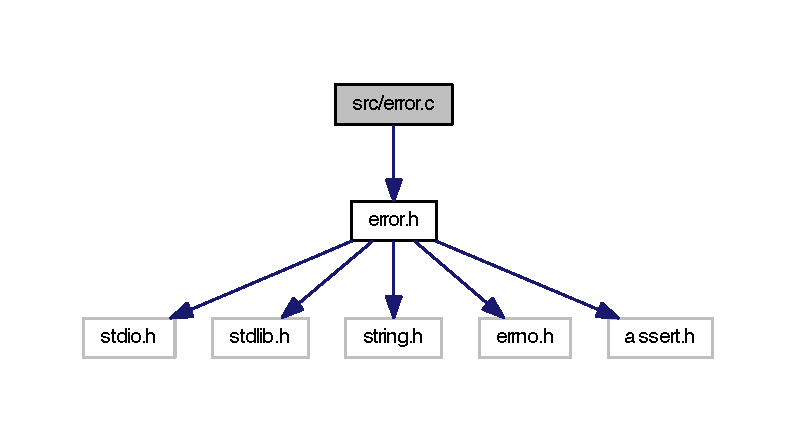
\includegraphics[width=350pt]{error_8c__incl}
\end{center}
\end{figure}
\subsection*{Functions}
\begin{DoxyCompactItemize}
\item 
void \hyperlink{error_8c_acf9a2facd46adb3083d36dbb8ea97521}{sys\+\_\+err} (const char $\ast$msg)
\begin{DoxyCompactList}\small\item\em if an error occured then print the error message and exit from program \end{DoxyCompactList}\end{DoxyCompactItemize}


\subsection{Detailed Description}
error handling 

\begin{DoxyAuthor}{Author}
M. Ozgan, \href{mailto:mozgan@mozgan.org}{\tt mozgan@mozgan.\+org} 
\end{DoxyAuthor}
\begin{DoxyVersion}{Version}
0.\+1 
\end{DoxyVersion}
\begin{DoxyDate}{Date}
23.\+08.\+2013 22\+:21\+:22 
\end{DoxyDate}
\begin{DoxyParagraph}{Compiler}
gcc (on Mac, and 4.\+4\+B\+S\+D) 
\end{DoxyParagraph}
\begin{DoxyParagraph}{Company}
T\+U Wien 
\end{DoxyParagraph}


\begin{DoxyRefDesc}{Bug}
\item[\hyperlink{bug__bug000001}{Bug}]none \end{DoxyRefDesc}
\begin{DoxyRefDesc}{Todo}
\item[\hyperlink{todo__todo000001}{Todo}]none \end{DoxyRefDesc}


Definition in file \hyperlink{error_8c_source}{error.\+c}.



\subsection{Function Documentation}
\hypertarget{error_8c_acf9a2facd46adb3083d36dbb8ea97521}{\index{error.\+c@{error.\+c}!sys\+\_\+err@{sys\+\_\+err}}
\index{sys\+\_\+err@{sys\+\_\+err}!error.\+c@{error.\+c}}
\subsubsection[{sys\+\_\+err}]{\setlength{\rightskip}{0pt plus 5cm}void sys\+\_\+err (
\begin{DoxyParamCaption}
\item[{const char $\ast$}]{msg}
\end{DoxyParamCaption}
)}}\label{error_8c_acf9a2facd46adb3083d36dbb8ea97521}


if an error occured then print the error message and exit from program 


\begin{DoxyParams}{Parameters}
{\em msg} & programmer message to print \\
\hline
\end{DoxyParams}


Definition at line \hyperlink{error_8c_source_l00035}{35} of file \hyperlink{error_8c_source}{error.\+c}.



Referenced by \hyperlink{udp_8c_source_l00060}{binding()}, \hyperlink{udp_8c_source_l00108}{close\+\_\+socket()}, \hyperlink{udp_8c_source_l00070}{communication()}, and \hyperlink{udp_8c_source_l00037}{make\+\_\+socket()}.


\hypertarget{error_8c_source}{\section{error.\+c}
\label{error_8c_source}\index{src/error.\+c@{src/error.\+c}}
}

\begin{DoxyCode}
00001 \textcolor{comment}{/*-}
00002 \textcolor{comment}{ * Copyright (c) 2013, mozgan.}
00003 \textcolor{comment}{ * All Rights Reserved with BSD License.}
00004 \textcolor{comment}{ * Read LICENSE file.}
00005 \textcolor{comment}{ */}
00006 
00022 \textcolor{comment}{/*}
00023 \textcolor{comment}{ *      @(#) src/error.c            TU Wien 23.08.2013}
00024 \textcolor{comment}{ *  $Id: error.c,v 0.1 23.08.2013 22:21:22 mozgan Exp $}
00025 \textcolor{comment}{ */}
00026 
00027 \textcolor{preprocessor}{#include "\hyperlink{error_8h}{error.h}"}
00028 
00034 \textcolor{keywordtype}{void}
\hypertarget{error_8c_source_l00035}{}\hyperlink{error_8h_a7c50c1dd9ff2f0d7d88bef6a99b4315c}{00035} \hyperlink{error_8c_acf9a2facd46adb3083d36dbb8ea97521}{sys\_err}(\textcolor{keyword}{const} \textcolor{keywordtype}{char} *msg)
00036 \{
00037         \textcolor{keywordflow}{if} (errno != 0)
00038                 (void)fprintf(stderr, \textcolor{stringliteral}{"Error: %s - %s\(\backslash\)n"}, msg, strerror(errno));
00039         \textcolor{keywordflow}{else}
00040                 (\textcolor{keywordtype}{void})fprintf(stderr, \textcolor{stringliteral}{"Error: %s\(\backslash\)n"}, msg);
00041 
00042         exit(EXIT\_FAILURE);
00043 \}
00044 
\end{DoxyCode}

\hypertarget{error_8h}{\section{src/error.h File Reference}
\label{error_8h}\index{src/error.\+h@{src/error.\+h}}
}


header file for error  


{\ttfamily \#include $<$stdio.\+h$>$}\\*
{\ttfamily \#include $<$stdlib.\+h$>$}\\*
{\ttfamily \#include $<$string.\+h$>$}\\*
{\ttfamily \#include $<$errno.\+h$>$}\\*
{\ttfamily \#include $<$assert.\+h$>$}\\*
Include dependency graph for error.\+h\+:\nopagebreak
\begin{figure}[H]
\begin{center}
\leavevmode
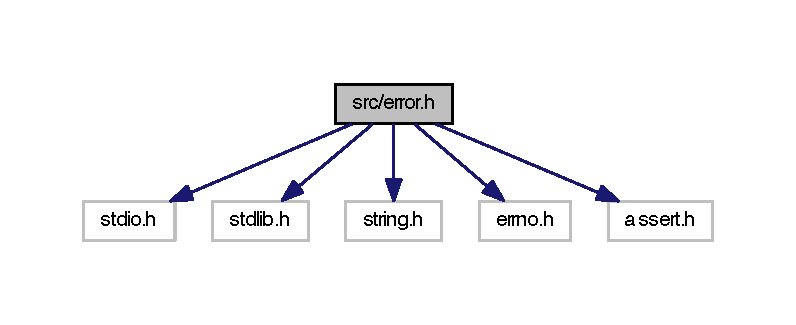
\includegraphics[width=350pt]{error_8h__incl}
\end{center}
\end{figure}
This graph shows which files directly or indirectly include this file\+:\nopagebreak
\begin{figure}[H]
\begin{center}
\leavevmode
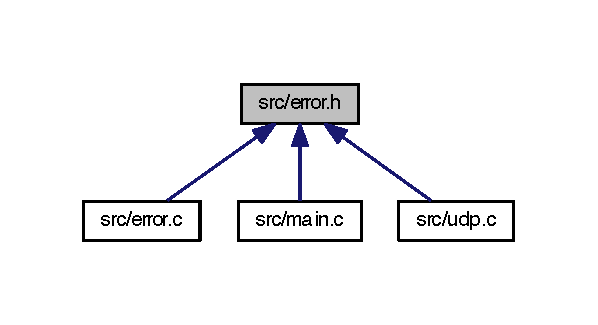
\includegraphics[width=287pt]{error_8h__dep__incl}
\end{center}
\end{figure}
\subsection*{Functions}
\begin{DoxyCompactItemize}
\item 
void \hyperlink{error_8h_a7c50c1dd9ff2f0d7d88bef6a99b4315c}{sys\+\_\+err} (const char $\ast$)
\begin{DoxyCompactList}\small\item\em if an error occured then print the error message and exit from program \end{DoxyCompactList}\end{DoxyCompactItemize}


\subsection{Detailed Description}
header file for error 

\begin{DoxyAuthor}{Author}
M. Ozgan, \href{mailto:mozgan@mozgan.org}{\tt mozgan@mozgan.\+org} 
\end{DoxyAuthor}
\begin{DoxyVersion}{Version}
0.\+1 
\end{DoxyVersion}
\begin{DoxyDate}{Date}
23.\+08.\+2013 22\+:20\+:44 
\end{DoxyDate}
\begin{DoxyParagraph}{Compiler}
gcc (on Mac, and 4.\+4\+B\+S\+D) 
\end{DoxyParagraph}
\begin{DoxyParagraph}{Company}
T\+U Wien 
\end{DoxyParagraph}


\begin{DoxyRefDesc}{Bug}
\item[\hyperlink{bug__bug000002}{Bug}]none \end{DoxyRefDesc}
\begin{DoxyRefDesc}{Todo}
\item[\hyperlink{todo__todo000002}{Todo}]none \end{DoxyRefDesc}


Definition in file \hyperlink{error_8h_source}{error.\+h}.



\subsection{Function Documentation}
\hypertarget{error_8h_a7c50c1dd9ff2f0d7d88bef6a99b4315c}{\index{error.\+h@{error.\+h}!sys\+\_\+err@{sys\+\_\+err}}
\index{sys\+\_\+err@{sys\+\_\+err}!error.\+h@{error.\+h}}
\subsubsection[{sys\+\_\+err}]{\setlength{\rightskip}{0pt plus 5cm}void sys\+\_\+err (
\begin{DoxyParamCaption}
\item[{const char $\ast$}]{msg}
\end{DoxyParamCaption}
)}}\label{error_8h_a7c50c1dd9ff2f0d7d88bef6a99b4315c}


if an error occured then print the error message and exit from program 


\begin{DoxyParams}{Parameters}
{\em msg} & programmer message to print \\
\hline
\end{DoxyParams}


Definition at line \hyperlink{error_8c_source_l00035}{35} of file \hyperlink{error_8c_source}{error.\+c}.



Referenced by \hyperlink{udp_8c_source_l00060}{binding()}, \hyperlink{udp_8c_source_l00108}{close\+\_\+socket()}, \hyperlink{udp_8c_source_l00070}{communication()}, and \hyperlink{udp_8c_source_l00037}{make\+\_\+socket()}.


\hypertarget{error_8h_source}{\section{error.\+h}
\label{error_8h_source}\index{src/error.\+h@{src/error.\+h}}
}

\begin{DoxyCode}
00001 \textcolor{comment}{/*-}
00002 \textcolor{comment}{ * Copyright (c) 2013, mozgan.}
00003 \textcolor{comment}{ * All Rights Reserved with BSD License.}
00004 \textcolor{comment}{ * Read LICENSE file.}
00005 \textcolor{comment}{ */}
00006 
00022 \textcolor{comment}{/*}
00023 \textcolor{comment}{ *      @(#) src/error.h                TU Wien 23.08.2013}
00024 \textcolor{comment}{ *  $Id: error.h,v 0.1 23.08.2013 22:20:44 mozgan Exp $}
00025 \textcolor{comment}{ */}
00026 
00027 \textcolor{preprocessor}{#ifndef \_\_ERROR\_H\_\_}
00028 \textcolor{preprocessor}{#define \_\_ERROR\_H\_\_}
00029 
00030 \textcolor{preprocessor}{#include <stdio.h>}
00031 \textcolor{preprocessor}{#include <stdlib.h>}
00032 \textcolor{preprocessor}{#include <string.h>}
00033 \textcolor{preprocessor}{#include <errno.h>}
00034 \textcolor{preprocessor}{#include <assert.h>}
00035 
00036 \textcolor{keywordtype}{void}            \hyperlink{error_8h_a7c50c1dd9ff2f0d7d88bef6a99b4315c}{sys\_err}(\textcolor{keyword}{const} \textcolor{keywordtype}{char} *);   \textcolor{comment}{/* system error */}
00037 
00038 
00039 
00040 \textcolor{preprocessor}{#endif }\textcolor{comment}{/* \_\_ERROR\_H\_\_ */}\textcolor{preprocessor}{}
00041 
\end{DoxyCode}

\hypertarget{main_8c}{\section{main.\+c File Reference}
\label{main_8c}\index{main.\+c@{main.\+c}}
}


main program  


{\ttfamily \#include $<$stdio.\+h$>$}\\*
{\ttfamily \#include $<$stdlib.\+h$>$}\\*
{\ttfamily \#include $<$string.\+h$>$}\\*
{\ttfamily \#include $<$avr/io.\+h$>$}\\*
{\ttfamily \#include $<$util/delay.\+h$>$}\\*
{\ttfamily \#include $<$include/common.\+h$>$}\\*
{\ttfamily \#include $<$board/freq.\+h$>$}\\*
{\ttfamily \#include $<$lib/buffer.\+h$>$}\\*
{\ttfamily \#include $<$driver/leds.\+h$>$}\\*
{\ttfamily \#include $<$device/enc28j60.\+h$>$}\\*
{\ttfamily \#include $<$driver/net.\+h$>$}\\*
{\ttfamily \#include $<$driver/icp.\+h$>$}\\*
Include dependency graph for main.\+c\+:
\nopagebreak
\begin{figure}[H]
\begin{center}
\leavevmode
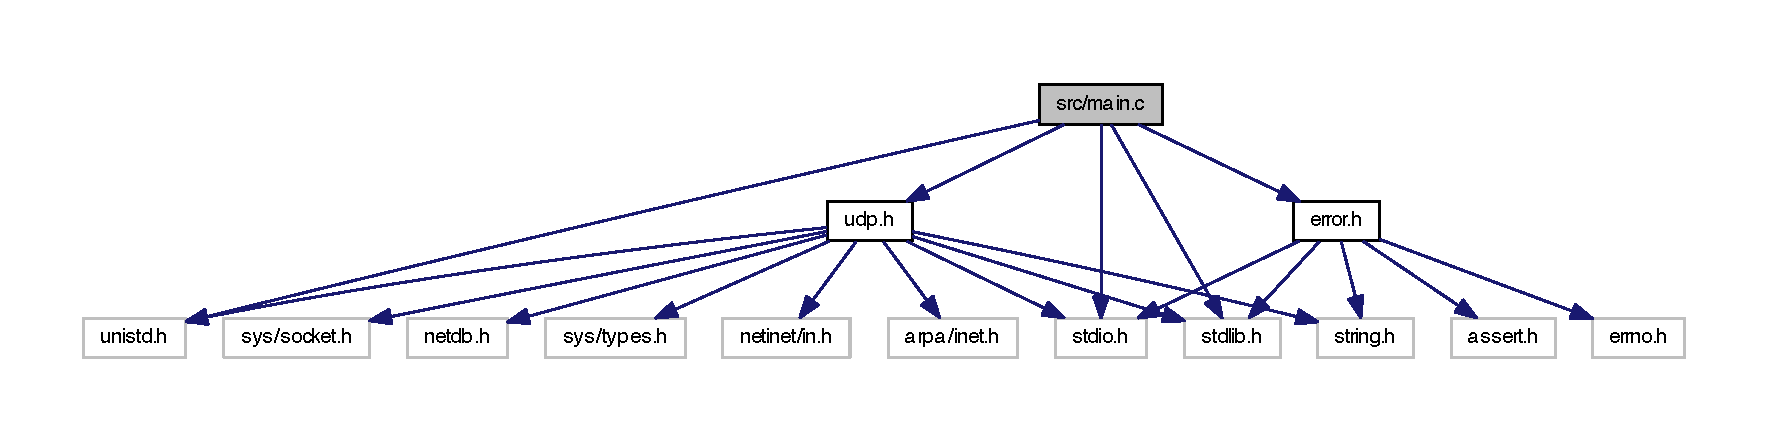
\includegraphics[width=350pt]{main_8c__incl}
\end{center}
\end{figure}
\subsection*{Macros}
\begin{DoxyCompactItemize}
\item 
\#define \hyperlink{main_8c_a6821bafc3c88dfb2e433a095df9940c6}{B\+U\+F\+\_\+\+S\+I\+Z\+E}~150
\end{DoxyCompactItemize}
\subsection*{Functions}
\begin{DoxyCompactItemize}
\item 
void \hyperlink{main_8c_aedb0558a93e7ad957d3186ba04578ca0}{trigger} (uint16\+\_\+t icr)
\begin{DoxyCompactList}\small\item\em return-\/function from input capture interrupt routine \end{DoxyCompactList}\item 
int \hyperlink{main_8c_a840291bc02cba5474a4cb46a9b9566fe}{main} (void)
\begin{DoxyCompactList}\small\item\em main function (program start) \end{DoxyCompactList}\end{DoxyCompactItemize}
\subsection*{Variables}
\begin{DoxyCompactItemize}
\item 
static uint8\+\_\+t \hyperlink{main_8c_aef549d19c508d258c21e95059b300d13}{buf} \mbox{[}\hyperlink{main_8c_a6821bafc3c88dfb2e433a095df9940c6}{B\+U\+F\+\_\+\+S\+I\+Z\+E}\mbox{]}
\item 
uint8\+\_\+t \hyperlink{main_8c_ae0177d7710b28f95720d54e2b1d37d65}{mymac} \mbox{[}6\mbox{]} = \{0xab,0xbc,0x6f,0x55,0x1c,0xc2\}
\item 
uint8\+\_\+t \hyperlink{main_8c_a60983d0ff040975723414a8f21375c77}{myip} \mbox{[}4\mbox{]} = \{192, 168, 0, 3\}
\item 
uint16\+\_\+t \hyperlink{main_8c_a2a1db0f1bf946876695219e06137df07}{myport} = 1200
\item 
volatile uint16\+\_\+t \hyperlink{main_8c_a1ec087735cb1d1e6da0c0a04fff747ba}{plen}
\item 
volatile uint16\+\_\+t \hyperlink{main_8c_a2e83eeb88a19fb6982fa4bce5235b0ad}{new}
\item 
volatile uint16\+\_\+t \hyperlink{main_8c_ae4e727681d08ae8c9618bb026716a532}{old}
\item 
volatile uint16\+\_\+t \hyperlink{main_8c_ace59d817931830cd94f04ac3f853bb76}{diff}
\item 
volatile float \hyperlink{main_8c_a74796ad69e9a5ee4a0448582ba5b1bb7}{freq}
\item 
volatile int \hyperlink{main_8c_a602b7b139bc6244cb09fedcdbb06e85e}{snd} = 0
\end{DoxyCompactItemize}


\subsection{Detailed Description}
main program 

\begin{DoxyAuthor}{Author}
M. Ozgan, \href{mailto:mozgan@mozgan.org}{\tt mozgan@mozgan.\+org} 
\end{DoxyAuthor}
\begin{DoxyVersion}{Version}
0.\+5 
\end{DoxyVersion}
\begin{DoxyDate}{Date}
19.\+08.\+2013 15\+:20\+:15 
\end{DoxyDate}
\begin{DoxyParagraph}{Compiler}
gcc (on Mac, and 4.\+4\+B\+S\+D) 
\end{DoxyParagraph}
\begin{DoxyParagraph}{Company}
T\+U Wien 
\end{DoxyParagraph}


\begin{DoxyRefDesc}{Bug}
\item[\hyperlink{bug__bug000019}{Bug}]
\begin{DoxyEnumerate}
\item signal has not readed! 
\end{DoxyEnumerate}\end{DoxyRefDesc}
\begin{DoxyRefDesc}{Todo}
\item[\hyperlink{todo__todo000019}{Todo}]none \end{DoxyRefDesc}


Definition in file \hyperlink{main_8c_source}{main.\+c}.



\subsection{Macro Definition Documentation}
\hypertarget{main_8c_a6821bafc3c88dfb2e433a095df9940c6}{\index{main.\+c@{main.\+c}!B\+U\+F\+\_\+\+S\+I\+Z\+E@{B\+U\+F\+\_\+\+S\+I\+Z\+E}}
\index{B\+U\+F\+\_\+\+S\+I\+Z\+E@{B\+U\+F\+\_\+\+S\+I\+Z\+E}!main.\+c@{main.\+c}}
\subsubsection[{B\+U\+F\+\_\+\+S\+I\+Z\+E}]{\setlength{\rightskip}{0pt plus 5cm}\#define B\+U\+F\+\_\+\+S\+I\+Z\+E~150}}\label{main_8c_a6821bafc3c88dfb2e433a095df9940c6}


Definition at line 43 of file main.\+c.



Referenced by main().



\subsection{Function Documentation}
\hypertarget{main_8c_a840291bc02cba5474a4cb46a9b9566fe}{\index{main.\+c@{main.\+c}!main@{main}}
\index{main@{main}!main.\+c@{main.\+c}}
\subsubsection[{main}]{\setlength{\rightskip}{0pt plus 5cm}int main (
\begin{DoxyParamCaption}
\item[{void}]{}
\end{DoxyParamCaption}
)}}\label{main_8c_a840291bc02cba5474a4cb46a9b9566fe}


main function (program start) 

\begin{DoxyReturn}{Returns}
returns zero if S\+U\+C\+C\+E\+S\+S, otherwise non-\/zero 
\end{DoxyReturn}


Definition at line 89 of file main.\+c.



References arp\+\_\+answer(), buf, B\+U\+F\+\_\+\+S\+I\+Z\+E, buffer\+\_\+init(), buffer\+\_\+medium(), diff, echo\+\_\+reply(), enc\+\_\+init(), enc\+\_\+init\+\_\+phy(), enc\+\_\+recv\+\_\+packet(), eth\+\_\+arp(), eth\+\_\+ip(), F\+\_\+\+C\+P\+U, freq, I\+C\+M\+P\+\_\+\+R\+E\+Q\+U\+E\+S\+T\+\_\+\+V, I\+C\+M\+P\+\_\+\+T\+Y\+P\+E\+\_\+\+P, icp\+\_\+init(), I\+P\+\_\+\+P\+R\+O\+T\+O\+\_\+\+I\+C\+M\+P\+\_\+\+V, I\+P\+\_\+\+P\+R\+O\+T\+O\+\_\+\+P, I\+P\+\_\+\+P\+R\+O\+T\+O\+\_\+\+U\+D\+P\+\_\+\+V, leds\+\_\+init(), L\+E\+N, myip, mymac, myport, net\+\_\+init(), plen, snd, trigger(), T\+R\+U\+E, and udp\+\_\+reply().



Here is the call graph for this function\+:
\nopagebreak
\begin{figure}[H]
\begin{center}
\leavevmode
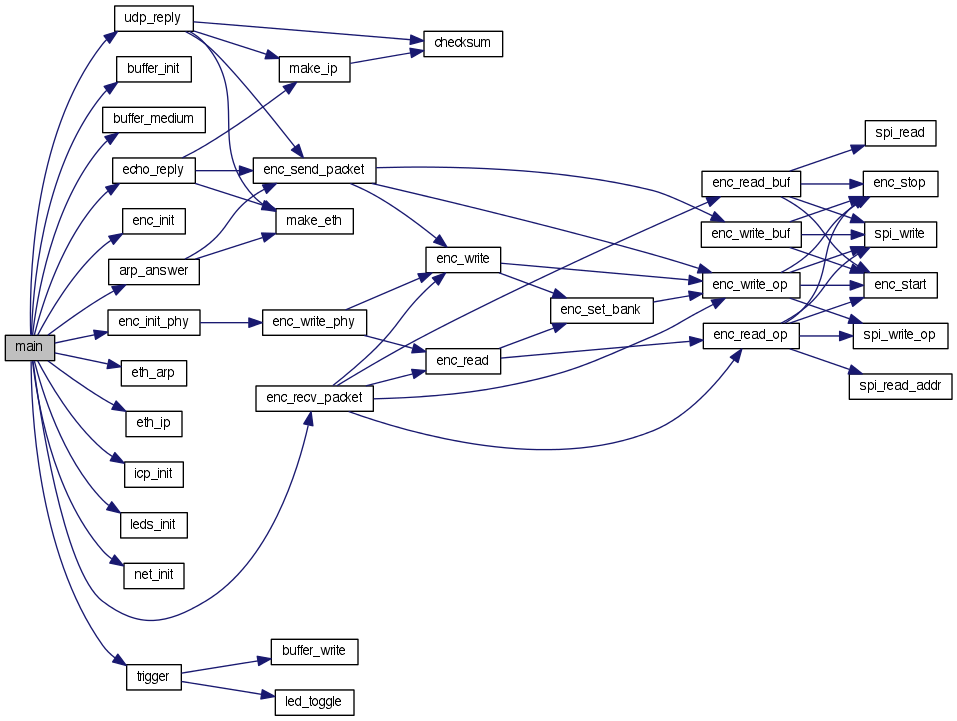
\includegraphics[width=350pt]{main_8c_a840291bc02cba5474a4cb46a9b9566fe_cgraph}
\end{center}
\end{figure}


\hypertarget{main_8c_aedb0558a93e7ad957d3186ba04578ca0}{\index{main.\+c@{main.\+c}!trigger@{trigger}}
\index{trigger@{trigger}!main.\+c@{main.\+c}}
\subsubsection[{trigger}]{\setlength{\rightskip}{0pt plus 5cm}void trigger (
\begin{DoxyParamCaption}
\item[{uint16\+\_\+t}]{icr}
\end{DoxyParamCaption}
)}}\label{main_8c_aedb0558a93e7ad957d3186ba04578ca0}


return-\/function from input capture interrupt routine 


\begin{DoxyParams}{Parameters}
{\em icr} & input capture timer state \\
\hline
\end{DoxyParams}


Definition at line 65 of file main.\+c.



References buffer\+\_\+write(), led\+\_\+toggle(), L\+E\+N, old, and snd.



Referenced by main().



Here is the call graph for this function\+:
\nopagebreak
\begin{figure}[H]
\begin{center}
\leavevmode
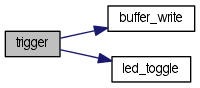
\includegraphics[width=222pt]{main_8c_aedb0558a93e7ad957d3186ba04578ca0_cgraph}
\end{center}
\end{figure}




\subsection{Variable Documentation}
\hypertarget{main_8c_aef549d19c508d258c21e95059b300d13}{\index{main.\+c@{main.\+c}!buf@{buf}}
\index{buf@{buf}!main.\+c@{main.\+c}}
\subsubsection[{buf}]{\setlength{\rightskip}{0pt plus 5cm}uint8\+\_\+t buf\mbox{[}{\bf B\+U\+F\+\_\+\+S\+I\+Z\+E}\mbox{]}\hspace{0.3cm}{\ttfamily [static]}}}\label{main_8c_aef549d19c508d258c21e95059b300d13}


Definition at line 45 of file main.\+c.



Referenced by checksum(), and main().

\hypertarget{main_8c_ace59d817931830cd94f04ac3f853bb76}{\index{main.\+c@{main.\+c}!diff@{diff}}
\index{diff@{diff}!main.\+c@{main.\+c}}
\subsubsection[{diff}]{\setlength{\rightskip}{0pt plus 5cm}volatile uint16\+\_\+t diff}}\label{main_8c_ace59d817931830cd94f04ac3f853bb76}


Definition at line 54 of file main.\+c.



Referenced by main().

\hypertarget{main_8c_a74796ad69e9a5ee4a0448582ba5b1bb7}{\index{main.\+c@{main.\+c}!freq@{freq}}
\index{freq@{freq}!main.\+c@{main.\+c}}
\subsubsection[{freq}]{\setlength{\rightskip}{0pt plus 5cm}volatile float freq}}\label{main_8c_a74796ad69e9a5ee4a0448582ba5b1bb7}


Definition at line 55 of file main.\+c.



Referenced by main().

\hypertarget{main_8c_a60983d0ff040975723414a8f21375c77}{\index{main.\+c@{main.\+c}!myip@{myip}}
\index{myip@{myip}!main.\+c@{main.\+c}}
\subsubsection[{myip}]{\setlength{\rightskip}{0pt plus 5cm}uint8\+\_\+t myip\mbox{[}4\mbox{]} = \{192, 168, 0, 3\}}}\label{main_8c_a60983d0ff040975723414a8f21375c77}


Definition at line 48 of file main.\+c.



Referenced by main().

\hypertarget{main_8c_ae0177d7710b28f95720d54e2b1d37d65}{\index{main.\+c@{main.\+c}!mymac@{mymac}}
\index{mymac@{mymac}!main.\+c@{main.\+c}}
\subsubsection[{mymac}]{\setlength{\rightskip}{0pt plus 5cm}uint8\+\_\+t mymac\mbox{[}6\mbox{]} = \{0xab,0xbc,0x6f,0x55,0x1c,0xc2\}}}\label{main_8c_ae0177d7710b28f95720d54e2b1d37d65}


Definition at line 47 of file main.\+c.



Referenced by main().

\hypertarget{main_8c_a2a1db0f1bf946876695219e06137df07}{\index{main.\+c@{main.\+c}!myport@{myport}}
\index{myport@{myport}!main.\+c@{main.\+c}}
\subsubsection[{myport}]{\setlength{\rightskip}{0pt plus 5cm}uint16\+\_\+t myport = 1200}}\label{main_8c_a2a1db0f1bf946876695219e06137df07}


Definition at line 49 of file main.\+c.



Referenced by main().

\hypertarget{main_8c_a2e83eeb88a19fb6982fa4bce5235b0ad}{\index{main.\+c@{main.\+c}!new@{new}}
\index{new@{new}!main.\+c@{main.\+c}}
\subsubsection[{new}]{\setlength{\rightskip}{0pt plus 5cm}volatile uint16\+\_\+t new}}\label{main_8c_a2e83eeb88a19fb6982fa4bce5235b0ad}


Definition at line 53 of file main.\+c.

\hypertarget{main_8c_ae4e727681d08ae8c9618bb026716a532}{\index{main.\+c@{main.\+c}!old@{old}}
\index{old@{old}!main.\+c@{main.\+c}}
\subsubsection[{old}]{\setlength{\rightskip}{0pt plus 5cm}volatile uint16\+\_\+t old}}\label{main_8c_ae4e727681d08ae8c9618bb026716a532}


Definition at line 53 of file main.\+c.



Referenced by trigger().

\hypertarget{main_8c_a1ec087735cb1d1e6da0c0a04fff747ba}{\index{main.\+c@{main.\+c}!plen@{plen}}
\index{plen@{plen}!main.\+c@{main.\+c}}
\subsubsection[{plen}]{\setlength{\rightskip}{0pt plus 5cm}volatile uint16\+\_\+t plen}}\label{main_8c_a1ec087735cb1d1e6da0c0a04fff747ba}


Definition at line 51 of file main.\+c.



Referenced by main().

\hypertarget{main_8c_a602b7b139bc6244cb09fedcdbb06e85e}{\index{main.\+c@{main.\+c}!snd@{snd}}
\index{snd@{snd}!main.\+c@{main.\+c}}
\subsubsection[{snd}]{\setlength{\rightskip}{0pt plus 5cm}volatile int snd = 0}}\label{main_8c_a602b7b139bc6244cb09fedcdbb06e85e}


Definition at line 57 of file main.\+c.



Referenced by main(), and trigger().


\hypertarget{main_8c_source}{\section{main.\+c}
\label{main_8c_source}\index{src/main.\+c@{src/main.\+c}}
}

\begin{DoxyCode}
00001 \textcolor{comment}{/*-}
00002 \textcolor{comment}{ * Copyright (c) 2013, mozgan.}
00003 \textcolor{comment}{ * All Rights Reserved with BSD License.}
00004 \textcolor{comment}{ * Read LICENSE file.}
00005 \textcolor{comment}{ */}
00006 
00022 \textcolor{comment}{/*}
00023 \textcolor{comment}{ *      @(#) src/main.c     TU Wien 23.08.2013}
00024 \textcolor{comment}{ *  $Id: main.c,v 0.1 23.08.2013 22:00:56 mozgan Exp $}
00025 \textcolor{comment}{ */}
00026 
00027 \textcolor{preprocessor}{#include <stdio.h>}
00028 \textcolor{preprocessor}{#include <stdlib.h>}
00029 \textcolor{preprocessor}{#include <unistd.h>}
00030 
00031 \textcolor{preprocessor}{#include "\hyperlink{udp_8h}{udp.h}"}
00032 \textcolor{preprocessor}{#include "\hyperlink{error_8h}{error.h}"}
00033 
\hypertarget{main_8c_source_l00034}{}\hyperlink{main_8c_adc0221a311d122f5c20b9ce7982f95ee}{00034} \textcolor{keyword}{const} \textcolor{keywordtype}{char}  *\hyperlink{main_8c_adc0221a311d122f5c20b9ce7982f95ee}{optstr} = \textcolor{stringliteral}{"h:p:"};                 
\hypertarget{main_8c_source_l00035}{}\hyperlink{main_8c_a8a8a6db7728221fbc910782969be77c2}{00035} \textcolor{keywordtype}{char}        *\hyperlink{main_8c_a8a8a6db7728221fbc910782969be77c2}{prg\_name} = \textcolor{stringliteral}{"<not yet set>"};    
00040 \textcolor{keywordtype}{void}
\hypertarget{main_8c_source_l00041}{}\hyperlink{main_8c_ae8605e2b78cd4a81b6c6b5c30cb7366a}{00041} \hyperlink{main_8c_ae8605e2b78cd4a81b6c6b5c30cb7366a}{usage}(\textcolor{keywordtype}{void})
00042 \{
00043         (void)fprintf(stdout, \textcolor{stringliteral}{"Usage: \(\backslash\)n"});
00044         (void)fprintf(stdout, \textcolor{stringliteral}{"\(\backslash\)t%s -h <hostname> -p <port>\(\backslash\)n"}, \hyperlink{main_8c_a8a8a6db7728221fbc910782969be77c2}{prg\_name});
00045         (void)fprintf(stdout, \textcolor{stringliteral}{"\(\backslash\)tExample: %s -h FreeBSD.local -p 32000\(\backslash\)n"}, 
      \hyperlink{main_8c_a8a8a6db7728221fbc910782969be77c2}{prg\_name});
00046 
00047         exit(EXIT\_FAILURE);
00048 \}
00049 
00050 
00059 \textcolor{keywordtype}{int}
\hypertarget{main_8c_source_l00060}{}\hyperlink{main_8c_a0ddf1224851353fc92bfbff6f499fa97}{00060} \hyperlink{main_8c_a0ddf1224851353fc92bfbff6f499fa97}{main}(\textcolor{keywordtype}{int} argc, \textcolor{keywordtype}{char} *argv[])
00061 \{
00062         \textcolor{keywordtype}{int}             ch;
00063         \textcolor{keywordtype}{int}             opt\_h, opt\_p;
00064         \textcolor{keywordtype}{char}            *end\_ptr;
00065         \textcolor{keywordtype}{char}            *hostname;      
00067         \hyperlink{main_8c_a8a8a6db7728221fbc910782969be77c2}{prg\_name} = argv[0];
00068         opt\_h = opt\_p = 0;
00069 
00070         \textcolor{comment}{/* it should be exactly 5 arguments */}
00071         \textcolor{keywordflow}{if} (argc != 5)
00072                 \hyperlink{main_8c_ae8605e2b78cd4a81b6c6b5c30cb7366a}{usage}();
00073 
00074         \textcolor{comment}{/* parse arguments */}
00075         \textcolor{keywordflow}{while}((ch = getopt(argc, argv, \hyperlink{main_8c_adc0221a311d122f5c20b9ce7982f95ee}{optstr})) != -1) \{
00076                 \textcolor{keywordflow}{switch}(ch) \{
00077                         \textcolor{keywordflow}{case} \textcolor{charliteral}{'h'}:
00078                                 hostname = optarg;
00079                                 printf (\textcolor{stringliteral}{"hostname: %s \(\backslash\)n"}, hostname);
00080                                 opt\_h = 1;
00081                                 \textcolor{keywordflow}{break};
00082                         \textcolor{keywordflow}{case} \textcolor{charliteral}{'p'}:
00083                                 \hyperlink{udp_8h_a54fac18369fc17e05c94bf0ab06ef7ac}{port\_nr} = (\textcolor{keywordtype}{unsigned} int)strtol(optarg, &end\_ptr, 10);
00084                                 printf (\textcolor{stringliteral}{"port number: %d\(\backslash\)n"}, \hyperlink{udp_8h_a54fac18369fc17e05c94bf0ab06ef7ac}{port\_nr});
00085                                 opt\_p = 1;
00086                                 \textcolor{keywordflow}{break};
00087                         \textcolor{keywordflow}{case} \textcolor{charliteral}{'?'}:
00088                                 \hyperlink{main_8c_ae8605e2b78cd4a81b6c6b5c30cb7366a}{usage}();
00089                                 exit(EXIT\_FAILURE);
00090                         \textcolor{keywordflow}{default}:
00091                                 abort();
00092                                 exit(EXIT\_FAILURE);
00093                 \}
00094         \}
00095         
00096         \textcolor{comment}{/* check the options correct gived */}
00097         \textcolor{keywordflow}{if} (!opt\_h || !opt\_p)
00098                 \hyperlink{main_8c_ae8605e2b78cd4a81b6c6b5c30cb7366a}{usage}();
00099 
00100         \textcolor{comment}{/* no more arguments accept */}
00101         \textcolor{keywordflow}{if} (optind != argc)
00102                 \hyperlink{main_8c_ae8605e2b78cd4a81b6c6b5c30cb7366a}{usage}();
00103         
00104         \hyperlink{udp_8c_af78c25c84b170f47fc907e752c1409b4}{make\_socket}(hostname, \hyperlink{udp_8h_a54fac18369fc17e05c94bf0ab06ef7ac}{port\_nr});           \textcolor{comment}{/* make the socket */}
00105         \hyperlink{udp_8c_a165726b24e152a113fdde7732b667b5f}{binding}();                           \textcolor{comment}{/* bind to host */}
00106         \hyperlink{udp_8c_a0b55dfe2fd6924e01624911af758ae03}{communication}();               \textcolor{comment}{/* send to host, recv from host */}
00107         \hyperlink{udp_8c_a1926d0bf833c9a35c53d2a2f601faa60}{close\_socket}();                         \textcolor{comment}{/* close the socket */}
00108         
00109         exit(EXIT\_SUCCESS);
00110 \}
00111 
\end{DoxyCode}

\hypertarget{udp_8c}{\section{src/udp.c File Reference}
\label{udp_8c}\index{src/udp.\+c@{src/udp.\+c}}
}


udp communication  


{\ttfamily \#include \char`\"{}udp.\+h\char`\"{}}\\*
{\ttfamily \#include \char`\"{}error.\+h\char`\"{}}\\*
Include dependency graph for udp.\+c\+:\nopagebreak
\begin{figure}[H]
\begin{center}
\leavevmode
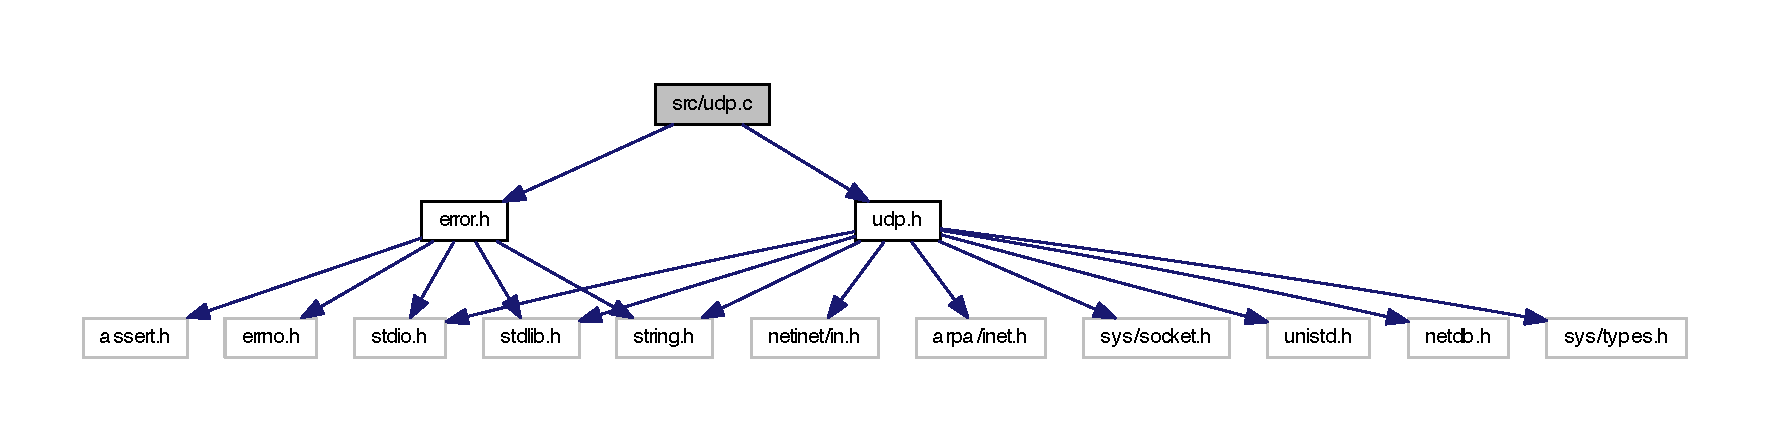
\includegraphics[width=350pt]{udp_8c__incl}
\end{center}
\end{figure}
\subsection*{Functions}
\begin{DoxyCompactItemize}
\item 
void \hyperlink{udp_8c_af78c25c84b170f47fc907e752c1409b4}{make\+\_\+socket} (const char $\ast$hostname, unsigned int port)
\begin{DoxyCompactList}\small\item\em make the socket \end{DoxyCompactList}\item 
void \hyperlink{udp_8c_a165726b24e152a113fdde7732b667b5f}{binding} (void)
\begin{DoxyCompactList}\small\item\em bind to host \end{DoxyCompactList}\item 
void \hyperlink{udp_8c_a0b55dfe2fd6924e01624911af758ae03}{communication} (void)
\begin{DoxyCompactList}\small\item\em make the communication with host (recv or send the datagrams) \end{DoxyCompactList}\item 
void \hyperlink{udp_8c_a1926d0bf833c9a35c53d2a2f601faa60}{close\+\_\+socket} (void)
\begin{DoxyCompactList}\small\item\em close the socket if not to use in future \end{DoxyCompactList}\end{DoxyCompactItemize}


\subsection{Detailed Description}
udp communication 

\begin{DoxyAuthor}{Author}
M. Ozgan, \href{mailto:mozgan@mozgan.org}{\tt mozgan@mozgan.\+org} 
\end{DoxyAuthor}
\begin{DoxyVersion}{Version}
0.\+1 
\end{DoxyVersion}
\begin{DoxyDate}{Date}
23.\+08.\+2013 22\+:01\+:48 
\end{DoxyDate}
\begin{DoxyParagraph}{Compiler}
gcc (on Mac, and 4.\+4\+B\+S\+D) 
\end{DoxyParagraph}
\begin{DoxyParagraph}{Company}
T\+U Wien 
\end{DoxyParagraph}


\begin{DoxyRefDesc}{Bug}
\item[\hyperlink{bug__bug000004}{Bug}]none \end{DoxyRefDesc}
\begin{DoxyRefDesc}{Todo}
\item[\hyperlink{todo__todo000004}{Todo}]none \end{DoxyRefDesc}


Definition in file \hyperlink{udp_8c_source}{udp.\+c}.



\subsection{Function Documentation}
\hypertarget{udp_8c_a165726b24e152a113fdde7732b667b5f}{\index{udp.\+c@{udp.\+c}!binding@{binding}}
\index{binding@{binding}!udp.\+c@{udp.\+c}}
\subsubsection[{binding}]{\setlength{\rightskip}{0pt plus 5cm}void binding (
\begin{DoxyParamCaption}
\item[{void}]{}
\end{DoxyParamCaption}
)}}\label{udp_8c_a165726b24e152a113fdde7732b667b5f}


bind to host 

bind to the socket 

Definition at line \hyperlink{udp_8c_source_l00060}{60} of file \hyperlink{udp_8c_source}{udp.\+c}.



References \hyperlink{udp_8h_source_l00058}{serv\+\_\+addr}, \hyperlink{udp_8h_source_l00060}{sock\+\_\+fd}, and \hyperlink{error_8c_source_l00035}{sys\+\_\+err()}.



Referenced by \hyperlink{main_8c_source_l00060}{main()}.



Here is the call graph for this function\+:\nopagebreak
\begin{figure}[H]
\begin{center}
\leavevmode
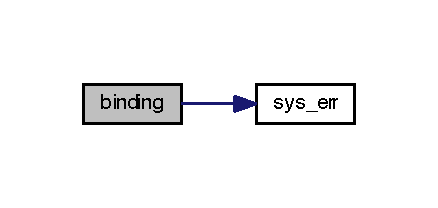
\includegraphics[width=210pt]{udp_8c_a165726b24e152a113fdde7732b667b5f_cgraph}
\end{center}
\end{figure}


\hypertarget{udp_8c_a1926d0bf833c9a35c53d2a2f601faa60}{\index{udp.\+c@{udp.\+c}!close\+\_\+socket@{close\+\_\+socket}}
\index{close\+\_\+socket@{close\+\_\+socket}!udp.\+c@{udp.\+c}}
\subsubsection[{close\+\_\+socket}]{\setlength{\rightskip}{0pt plus 5cm}void close\+\_\+socket (
\begin{DoxyParamCaption}
\item[{void}]{}
\end{DoxyParamCaption}
)}}\label{udp_8c_a1926d0bf833c9a35c53d2a2f601faa60}


close the socket if not to use in future 

close the open socket 

Definition at line \hyperlink{udp_8c_source_l00108}{108} of file \hyperlink{udp_8c_source}{udp.\+c}.



References \hyperlink{udp_8h_source_l00060}{sock\+\_\+fd}, and \hyperlink{error_8c_source_l00035}{sys\+\_\+err()}.



Referenced by \hyperlink{main_8c_source_l00060}{main()}.



Here is the call graph for this function\+:\nopagebreak
\begin{figure}[H]
\begin{center}
\leavevmode
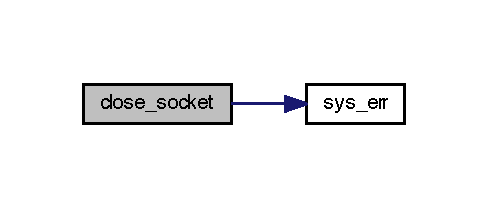
\includegraphics[width=234pt]{udp_8c_a1926d0bf833c9a35c53d2a2f601faa60_cgraph}
\end{center}
\end{figure}


\hypertarget{udp_8c_a0b55dfe2fd6924e01624911af758ae03}{\index{udp.\+c@{udp.\+c}!communication@{communication}}
\index{communication@{communication}!udp.\+c@{udp.\+c}}
\subsubsection[{communication}]{\setlength{\rightskip}{0pt plus 5cm}void communication (
\begin{DoxyParamCaption}
\item[{void}]{}
\end{DoxyParamCaption}
)}}\label{udp_8c_a0b55dfe2fd6924e01624911af758ae03}


make the communication with host (recv or send the datagrams) 

communication 

Definition at line \hyperlink{udp_8c_source_l00070}{70} of file \hyperlink{udp_8c_source}{udp.\+c}.



References \hyperlink{udp_8h_source_l00057}{dest\+\_\+addr}, \hyperlink{udp_8h_source_l00060}{sock\+\_\+fd}, and \hyperlink{error_8c_source_l00035}{sys\+\_\+err()}.



Referenced by \hyperlink{main_8c_source_l00060}{main()}.



Here is the call graph for this function\+:\nopagebreak
\begin{figure}[H]
\begin{center}
\leavevmode
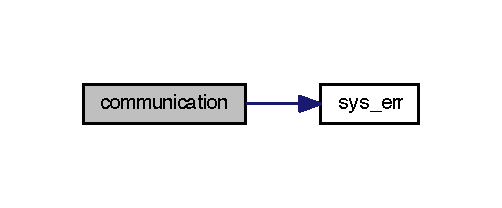
\includegraphics[width=241pt]{udp_8c_a0b55dfe2fd6924e01624911af758ae03_cgraph}
\end{center}
\end{figure}


\hypertarget{udp_8c_af78c25c84b170f47fc907e752c1409b4}{\index{udp.\+c@{udp.\+c}!make\+\_\+socket@{make\+\_\+socket}}
\index{make\+\_\+socket@{make\+\_\+socket}!udp.\+c@{udp.\+c}}
\subsubsection[{make\+\_\+socket}]{\setlength{\rightskip}{0pt plus 5cm}void make\+\_\+socket (
\begin{DoxyParamCaption}
\item[{const char $\ast$}]{hostname, }
\item[{unsigned int}]{port}
\end{DoxyParamCaption}
)}}\label{udp_8c_af78c25c84b170f47fc907e752c1409b4}


make the socket 


\begin{DoxyParams}{Parameters}
{\em hostname} & get the hostname \\
\hline
{\em port} & port number to connection \\
\hline
\end{DoxyParams}


Definition at line \hyperlink{udp_8c_source_l00037}{37} of file \hyperlink{udp_8c_source}{udp.\+c}.



References \hyperlink{udp_8h_source_l00057}{dest\+\_\+addr}, \hyperlink{udp_8h_source_l00055}{h\+\_\+name}, \hyperlink{udp_8h_source_l00058}{serv\+\_\+addr}, \hyperlink{udp_8h_source_l00060}{sock\+\_\+fd}, \hyperlink{error_8c_source_l00035}{sys\+\_\+err()}, and \hyperlink{udp_8h_source_l00045}{u\+\_\+long}.



Referenced by \hyperlink{main_8c_source_l00060}{main()}.



Here is the call graph for this function\+:\nopagebreak
\begin{figure}[H]
\begin{center}
\leavevmode
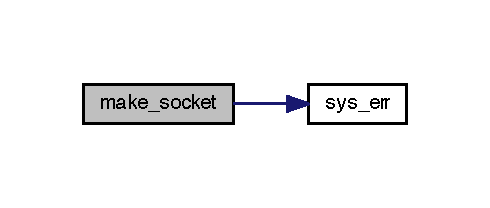
\includegraphics[width=235pt]{udp_8c_af78c25c84b170f47fc907e752c1409b4_cgraph}
\end{center}
\end{figure}



\hypertarget{udp_8c_source}{\section{udp.\+c}
\label{udp_8c_source}\index{src/udp.\+c@{src/udp.\+c}}
}

\begin{DoxyCode}
00001 \textcolor{comment}{/*-}
00002 \textcolor{comment}{ * Copyright (c) 2013, mozgan.}
00003 \textcolor{comment}{ * All Rights Reserved with BSD License.}
00004 \textcolor{comment}{ * Read LICENSE file.}
00005 \textcolor{comment}{ */}
00006 
00022 \textcolor{comment}{/*}
00023 \textcolor{comment}{ *      @(#) src/udp.c      TU Wien 23.08.2013}
00024 \textcolor{comment}{ *  $Id: udp.c,v 0.1 23.08.2013 22:01:48 mozgan Exp $}
00025 \textcolor{comment}{ */}
00026 
00027 \textcolor{preprocessor}{#include "\hyperlink{udp_8h}{udp.h}"}
00028 \textcolor{preprocessor}{#include "\hyperlink{error_8h}{error.h}"}
00029 
00036 \textcolor{keywordtype}{void}
\hypertarget{udp_8c_source_l00037}{}\hyperlink{udp_8h_af62eaae41c3f2e3caa57d3735a0ec053}{00037} \hyperlink{udp_8c_af78c25c84b170f47fc907e752c1409b4}{make\_socket}(\textcolor{keyword}{const} \textcolor{keywordtype}{char} *hostname, \textcolor{keywordtype}{unsigned} \textcolor{keywordtype}{int} port)
00038 \{
00039         memset(&\hyperlink{udp_8h_a072220ecebc8a6044aca4afa78eefebd}{dest\_addr}, 0, \textcolor{keyword}{sizeof}(\hyperlink{udp_8h_a072220ecebc8a6044aca4afa78eefebd}{dest\_addr}));
00040 
00041         \hyperlink{udp_8h_aecc6f69775dc6fdfbfde27f60b417932}{h\_name} = gethostbyname(hostname);
00042 
00043         \hyperlink{udp_8h_a072220ecebc8a6044aca4afa78eefebd}{dest\_addr}.sin\_family = AF\_INET;
00044         \hyperlink{udp_8h_a072220ecebc8a6044aca4afa78eefebd}{dest\_addr}.sin\_addr.s\_addr = *(\hyperlink{udp_8h_aaf12d2783d89167480b76853da8ba5e1}{u\_long} *)\hyperlink{udp_8h_aecc6f69775dc6fdfbfde27f60b417932}{h\_name}->h\_addr\_list[0];
00045         \hyperlink{udp_8h_a072220ecebc8a6044aca4afa78eefebd}{dest\_addr}.sin\_port = htons(port);
00046 
00047         \hyperlink{udp_8h_ac724fe70ae8af2d1406927ee7b574a1b}{serv\_addr}.sin\_family = AF\_INET;
00048         \hyperlink{udp_8h_ac724fe70ae8af2d1406927ee7b574a1b}{serv\_addr}.sin\_addr.s\_addr = htonl(INADDR\_ANY);
00049         \hyperlink{udp_8h_ac724fe70ae8af2d1406927ee7b574a1b}{serv\_addr}.sin\_port = htons(port);
00050         memset(&\hyperlink{udp_8h_ac724fe70ae8af2d1406927ee7b574a1b}{serv\_addr}.sin\_zero, 0, \textcolor{keyword}{sizeof}(\hyperlink{udp_8h_ac724fe70ae8af2d1406927ee7b574a1b}{serv\_addr}.sin\_zero));
00051         
00052         \textcolor{keywordflow}{if} ((\hyperlink{udp_8h_a514331e6141a28289f8ddead55eadebd}{sock\_fd} = socket(AF\_INET, SOCK\_DGRAM, IPPROTO\_UDP)) == -1)
00053                 \hyperlink{error_8c_acf9a2facd46adb3083d36dbb8ea97521}{sys\_err}(\textcolor{stringliteral}{"creating socket failed"});
00054 \}
00055 
00059 \textcolor{keywordtype}{void}
\hypertarget{udp_8c_source_l00060}{}\hyperlink{udp_8h_a165726b24e152a113fdde7732b667b5f}{00060} \hyperlink{udp_8c_a165726b24e152a113fdde7732b667b5f}{binding}(\textcolor{keywordtype}{void})
00061 \{
00062         \textcolor{keywordflow}{if} (bind(\hyperlink{udp_8h_a514331e6141a28289f8ddead55eadebd}{sock\_fd}, (\textcolor{keyword}{struct} sockaddr *)&\hyperlink{udp_8h_ac724fe70ae8af2d1406927ee7b574a1b}{serv\_addr}, \textcolor{keyword}{sizeof}(
      \hyperlink{udp_8h_ac724fe70ae8af2d1406927ee7b574a1b}{serv\_addr})))
00063                 \hyperlink{error_8c_acf9a2facd46adb3083d36dbb8ea97521}{sys\_err}(\textcolor{stringliteral}{"bind socket failed"});
00064 \}
00065 
00069 \textcolor{keywordtype}{void}
\hypertarget{udp_8c_source_l00070}{}\hyperlink{udp_8h_a0b55dfe2fd6924e01624911af758ae03}{00070} \hyperlink{udp_8c_a0b55dfe2fd6924e01624911af758ae03}{communication}(\textcolor{keywordtype}{void})
00071 \{
00072         \textcolor{keywordtype}{int}             len;
00073         \textcolor{keywordtype}{char}            buf[BUFSIZ];
00074         socklen\_t       sin\_size;
00075         
00076 
00077         \textcolor{comment}{/*** send to client ***/}
00078 
00079         \textcolor{keywordflow}{if} (strcpy(buf, \textcolor{stringliteral}{"start"}) == NULL)
00080                 \hyperlink{error_8c_acf9a2facd46adb3083d36dbb8ea97521}{sys\_err}(\textcolor{stringliteral}{"copy the string to buffer failed"});
00081         
00082         (void)fprintf(stdout, \textcolor{stringliteral}{"sending: %s\(\backslash\)n"}, buf);
00083 
00084         \textcolor{keywordflow}{if} (sendto(\hyperlink{udp_8h_a514331e6141a28289f8ddead55eadebd}{sock\_fd}, buf, strlen(buf), 0, (\textcolor{keyword}{struct} sockaddr *)&
      \hyperlink{udp_8h_a072220ecebc8a6044aca4afa78eefebd}{dest\_addr}, \textcolor{keyword}{sizeof}(\textcolor{keyword}{struct} sockaddr)) == -1)
00085                 \hyperlink{error_8c_acf9a2facd46adb3083d36dbb8ea97521}{sys\_err}(\textcolor{stringliteral}{"sendto failed"});
00086 
00087 
00088 
00089         \textcolor{comment}{/*** receive from client ***/}
00090 
00091         sin\_size = (socklen\_t)\textcolor{keyword}{sizeof}(\textcolor{keyword}{struct} sockaddr\_in);
00092         (void)fprintf(stdout, \textcolor{stringliteral}{"waiting for packet ...\(\backslash\)n"});
00093 
00094         \textcolor{keywordflow}{if}((len = recvfrom(\hyperlink{udp_8h_a514331e6141a28289f8ddead55eadebd}{sock\_fd}, buf, BUFSIZ, 0, (\textcolor{keyword}{struct} sockaddr *)&
      \hyperlink{udp_8h_a072220ecebc8a6044aca4afa78eefebd}{dest\_addr}, &sin\_size)) == -1) 
00095                 \hyperlink{error_8c_acf9a2facd46adb3083d36dbb8ea97521}{sys\_err}(\textcolor{stringliteral}{"recvfrom failed"});
00096         
00097         (void)fprintf(stdout, \textcolor{stringliteral}{"received packet from %s: "}, inet\_ntoa(\hyperlink{udp_8h_a072220ecebc8a6044aca4afa78eefebd}{dest\_addr}.sin\_addr));
00098 
00099         buf[len] = \textcolor{charliteral}{'\(\backslash\)0'};
00100         (void)fprintf(stdout, \textcolor{stringliteral}{"%s Hz\(\backslash\)n"}, buf);
00101 
00102 \}
00103 
00107 \textcolor{keywordtype}{void}
\hypertarget{udp_8c_source_l00108}{}\hyperlink{udp_8h_a1926d0bf833c9a35c53d2a2f601faa60}{00108} \hyperlink{udp_8c_a1926d0bf833c9a35c53d2a2f601faa60}{close\_socket}(\textcolor{keywordtype}{void})
00109 \{
00110         \textcolor{keywordflow}{if} (close(\hyperlink{udp_8h_a514331e6141a28289f8ddead55eadebd}{sock\_fd}) == -1)
00111                 \hyperlink{error_8c_acf9a2facd46adb3083d36dbb8ea97521}{sys\_err}(\textcolor{stringliteral}{"close socket failed"});
00112 \}
00113 
\end{DoxyCode}

\hypertarget{udp_8h}{\section{src/udp.h File Reference}
\label{udp_8h}\index{src/udp.\+h@{src/udp.\+h}}
}


header file for udp communication  


{\ttfamily \#include $<$stdio.\+h$>$}\\*
{\ttfamily \#include $<$stdlib.\+h$>$}\\*
{\ttfamily \#include $<$string.\+h$>$}\\*
{\ttfamily \#include $<$unistd.\+h$>$}\\*
{\ttfamily \#include $<$netdb.\+h$>$}\\*
{\ttfamily \#include $<$sys/types.\+h$>$}\\*
{\ttfamily \#include $<$netinet/in.\+h$>$}\\*
{\ttfamily \#include $<$arpa/inet.\+h$>$}\\*
{\ttfamily \#include $<$sys/socket.\+h$>$}\\*
Include dependency graph for udp.\+h\+:\nopagebreak
\begin{figure}[H]
\begin{center}
\leavevmode
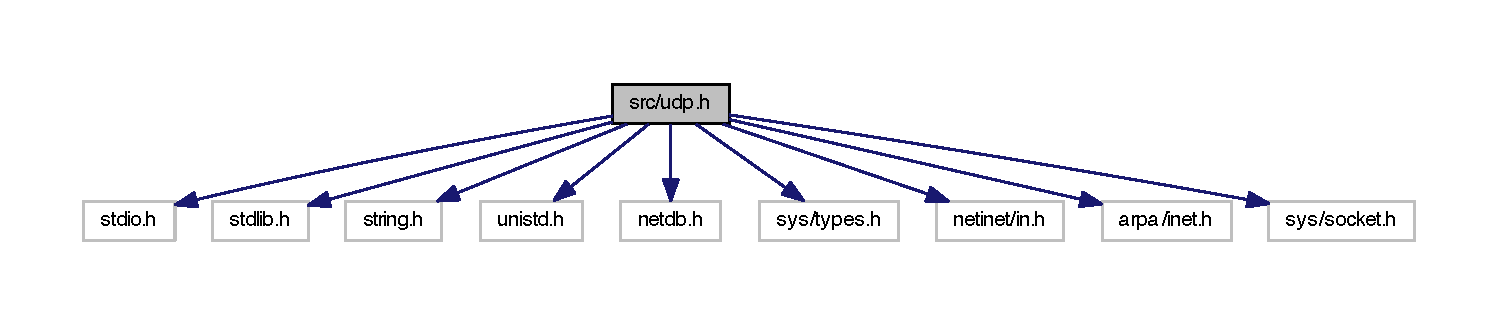
\includegraphics[width=350pt]{udp_8h__incl}
\end{center}
\end{figure}
This graph shows which files directly or indirectly include this file\+:\nopagebreak
\begin{figure}[H]
\begin{center}
\leavevmode
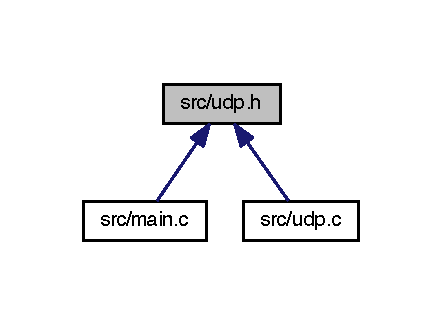
\includegraphics[width=212pt]{udp_8h__dep__incl}
\end{center}
\end{figure}
\subsection*{Macros}
\begin{DoxyCompactItemize}
\item 
\#define \hyperlink{udp_8h_aaf12d2783d89167480b76853da8ba5e1}{u\+\_\+long}~unsigned long
\item 
\#define \hyperlink{udp_8h_a4d04a8261523c8f3473946257c12ce5b}{h\+\_\+addr}~h\+\_\+addr\+\_\+list\mbox{[}0\mbox{]}
\end{DoxyCompactItemize}
\subsection*{Functions}
\begin{DoxyCompactItemize}
\item 
void \hyperlink{udp_8h_af62eaae41c3f2e3caa57d3735a0ec053}{make\+\_\+socket} (const char $\ast$, unsigned int)
\begin{DoxyCompactList}\small\item\em make the socket \end{DoxyCompactList}\item 
void \hyperlink{udp_8h_a165726b24e152a113fdde7732b667b5f}{binding} (void)
\begin{DoxyCompactList}\small\item\em bind to host \end{DoxyCompactList}\item 
void \hyperlink{udp_8h_a0b55dfe2fd6924e01624911af758ae03}{communication} (void)
\begin{DoxyCompactList}\small\item\em make the communication with host (recv or send the datagrams) \end{DoxyCompactList}\item 
void \hyperlink{udp_8h_a1926d0bf833c9a35c53d2a2f601faa60}{close\+\_\+socket} (void)
\begin{DoxyCompactList}\small\item\em close the socket if not to use in future \end{DoxyCompactList}\end{DoxyCompactItemize}
\subsection*{Variables}
\begin{DoxyCompactItemize}
\item 
struct hostent $\ast$ \hyperlink{udp_8h_aecc6f69775dc6fdfbfde27f60b417932}{h\+\_\+name}
\item 
struct sockaddr\+\_\+in \hyperlink{udp_8h_a072220ecebc8a6044aca4afa78eefebd}{dest\+\_\+addr}
\item 
struct sockaddr\+\_\+in \hyperlink{udp_8h_ac724fe70ae8af2d1406927ee7b574a1b}{serv\+\_\+addr}
\item 
int \hyperlink{udp_8h_a514331e6141a28289f8ddead55eadebd}{sock\+\_\+fd}
\item 
unsigned int \hyperlink{udp_8h_a54fac18369fc17e05c94bf0ab06ef7ac}{port\+\_\+nr}
\end{DoxyCompactItemize}


\subsection{Detailed Description}
header file for udp communication 

\begin{DoxyAuthor}{Author}
M. Ozgan, \href{mailto:mozgan@mozgan.org}{\tt mozgan@mozgan.\+org} 
\end{DoxyAuthor}
\begin{DoxyVersion}{Version}
0.\+1 
\end{DoxyVersion}
\begin{DoxyDate}{Date}
23.\+08.\+2013 22\+:02\+:31 
\end{DoxyDate}
\begin{DoxyParagraph}{Compiler}
gcc (on Mac, and 4.\+4\+B\+S\+D) 
\end{DoxyParagraph}
\begin{DoxyParagraph}{Company}
T\+U Wien 
\end{DoxyParagraph}


\begin{DoxyRefDesc}{Bug}
\item[\hyperlink{bug__bug000005}{Bug}]none \end{DoxyRefDesc}
\begin{DoxyRefDesc}{Todo}
\item[\hyperlink{todo__todo000005}{Todo}]none \end{DoxyRefDesc}


Definition in file \hyperlink{udp_8h_source}{udp.\+h}.



\subsection{Macro Definition Documentation}
\hypertarget{udp_8h_a4d04a8261523c8f3473946257c12ce5b}{\index{udp.\+h@{udp.\+h}!h\+\_\+addr@{h\+\_\+addr}}
\index{h\+\_\+addr@{h\+\_\+addr}!udp.\+h@{udp.\+h}}
\subsubsection[{h\+\_\+addr}]{\setlength{\rightskip}{0pt plus 5cm}\#define h\+\_\+addr~h\+\_\+addr\+\_\+list\mbox{[}0\mbox{]}}}\label{udp_8h_a4d04a8261523c8f3473946257c12ce5b}


Definition at line \hyperlink{udp_8h_source_l00052}{52} of file \hyperlink{udp_8h_source}{udp.\+h}.

\hypertarget{udp_8h_aaf12d2783d89167480b76853da8ba5e1}{\index{udp.\+h@{udp.\+h}!u\+\_\+long@{u\+\_\+long}}
\index{u\+\_\+long@{u\+\_\+long}!udp.\+h@{udp.\+h}}
\subsubsection[{u\+\_\+long}]{\setlength{\rightskip}{0pt plus 5cm}\#define u\+\_\+long~unsigned long}}\label{udp_8h_aaf12d2783d89167480b76853da8ba5e1}


Definition at line \hyperlink{udp_8h_source_l00045}{45} of file \hyperlink{udp_8h_source}{udp.\+h}.



Referenced by \hyperlink{udp_8c_source_l00037}{make\+\_\+socket()}.



\subsection{Function Documentation}
\hypertarget{udp_8h_a165726b24e152a113fdde7732b667b5f}{\index{udp.\+h@{udp.\+h}!binding@{binding}}
\index{binding@{binding}!udp.\+h@{udp.\+h}}
\subsubsection[{binding}]{\setlength{\rightskip}{0pt plus 5cm}void binding (
\begin{DoxyParamCaption}
\item[{void}]{}
\end{DoxyParamCaption}
)}}\label{udp_8h_a165726b24e152a113fdde7732b667b5f}


bind to host 

bind to the socket 

Definition at line \hyperlink{udp_8c_source_l00060}{60} of file \hyperlink{udp_8c_source}{udp.\+c}.



References \hyperlink{udp_8h_source_l00058}{serv\+\_\+addr}, \hyperlink{udp_8h_source_l00060}{sock\+\_\+fd}, and \hyperlink{error_8c_source_l00035}{sys\+\_\+err()}.



Referenced by \hyperlink{main_8c_source_l00060}{main()}.



Here is the call graph for this function\+:\nopagebreak
\begin{figure}[H]
\begin{center}
\leavevmode
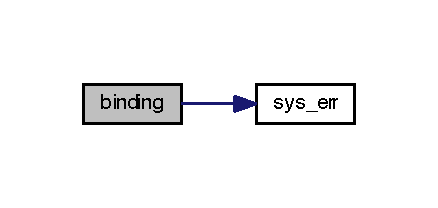
\includegraphics[width=210pt]{udp_8h_a165726b24e152a113fdde7732b667b5f_cgraph}
\end{center}
\end{figure}


\hypertarget{udp_8h_a1926d0bf833c9a35c53d2a2f601faa60}{\index{udp.\+h@{udp.\+h}!close\+\_\+socket@{close\+\_\+socket}}
\index{close\+\_\+socket@{close\+\_\+socket}!udp.\+h@{udp.\+h}}
\subsubsection[{close\+\_\+socket}]{\setlength{\rightskip}{0pt plus 5cm}void close\+\_\+socket (
\begin{DoxyParamCaption}
\item[{void}]{}
\end{DoxyParamCaption}
)}}\label{udp_8h_a1926d0bf833c9a35c53d2a2f601faa60}


close the socket if not to use in future 

close the open socket 

Definition at line \hyperlink{udp_8c_source_l00108}{108} of file \hyperlink{udp_8c_source}{udp.\+c}.



References \hyperlink{udp_8h_source_l00060}{sock\+\_\+fd}, and \hyperlink{error_8c_source_l00035}{sys\+\_\+err()}.



Referenced by \hyperlink{main_8c_source_l00060}{main()}.



Here is the call graph for this function\+:\nopagebreak
\begin{figure}[H]
\begin{center}
\leavevmode
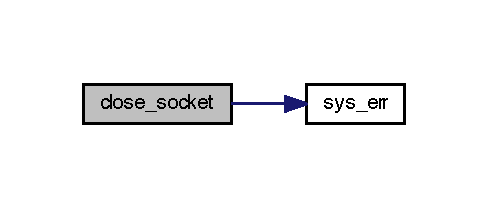
\includegraphics[width=234pt]{udp_8h_a1926d0bf833c9a35c53d2a2f601faa60_cgraph}
\end{center}
\end{figure}


\hypertarget{udp_8h_a0b55dfe2fd6924e01624911af758ae03}{\index{udp.\+h@{udp.\+h}!communication@{communication}}
\index{communication@{communication}!udp.\+h@{udp.\+h}}
\subsubsection[{communication}]{\setlength{\rightskip}{0pt plus 5cm}void communication (
\begin{DoxyParamCaption}
\item[{void}]{}
\end{DoxyParamCaption}
)}}\label{udp_8h_a0b55dfe2fd6924e01624911af758ae03}


make the communication with host (recv or send the datagrams) 

communication 

Definition at line \hyperlink{udp_8c_source_l00070}{70} of file \hyperlink{udp_8c_source}{udp.\+c}.



References \hyperlink{udp_8h_source_l00057}{dest\+\_\+addr}, \hyperlink{udp_8h_source_l00060}{sock\+\_\+fd}, and \hyperlink{error_8c_source_l00035}{sys\+\_\+err()}.



Referenced by \hyperlink{main_8c_source_l00060}{main()}.



Here is the call graph for this function\+:\nopagebreak
\begin{figure}[H]
\begin{center}
\leavevmode
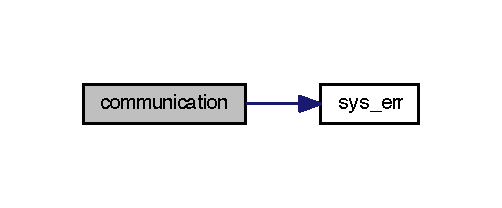
\includegraphics[width=241pt]{udp_8h_a0b55dfe2fd6924e01624911af758ae03_cgraph}
\end{center}
\end{figure}


\hypertarget{udp_8h_af62eaae41c3f2e3caa57d3735a0ec053}{\index{udp.\+h@{udp.\+h}!make\+\_\+socket@{make\+\_\+socket}}
\index{make\+\_\+socket@{make\+\_\+socket}!udp.\+h@{udp.\+h}}
\subsubsection[{make\+\_\+socket}]{\setlength{\rightskip}{0pt plus 5cm}void make\+\_\+socket (
\begin{DoxyParamCaption}
\item[{const char $\ast$}]{hostname, }
\item[{unsigned int}]{port}
\end{DoxyParamCaption}
)}}\label{udp_8h_af62eaae41c3f2e3caa57d3735a0ec053}


make the socket 

make a socket


\begin{DoxyParams}{Parameters}
{\em hostname} & get the hostname \\
\hline
{\em port} & port number to connection \\
\hline
\end{DoxyParams}


Definition at line \hyperlink{udp_8c_source_l00037}{37} of file \hyperlink{udp_8c_source}{udp.\+c}.



References \hyperlink{udp_8h_source_l00057}{dest\+\_\+addr}, \hyperlink{udp_8h_source_l00055}{h\+\_\+name}, \hyperlink{udp_8h_source_l00058}{serv\+\_\+addr}, \hyperlink{udp_8h_source_l00060}{sock\+\_\+fd}, \hyperlink{error_8c_source_l00035}{sys\+\_\+err()}, and \hyperlink{udp_8h_source_l00045}{u\+\_\+long}.



Referenced by \hyperlink{main_8c_source_l00060}{main()}.



Here is the call graph for this function\+:\nopagebreak
\begin{figure}[H]
\begin{center}
\leavevmode
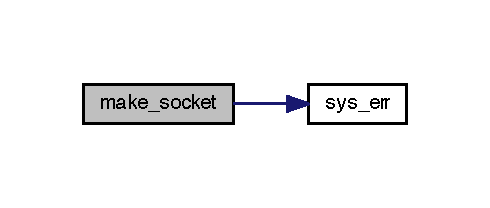
\includegraphics[width=235pt]{udp_8h_af62eaae41c3f2e3caa57d3735a0ec053_cgraph}
\end{center}
\end{figure}




\subsection{Variable Documentation}
\hypertarget{udp_8h_a072220ecebc8a6044aca4afa78eefebd}{\index{udp.\+h@{udp.\+h}!dest\+\_\+addr@{dest\+\_\+addr}}
\index{dest\+\_\+addr@{dest\+\_\+addr}!udp.\+h@{udp.\+h}}
\subsubsection[{dest\+\_\+addr}]{\setlength{\rightskip}{0pt plus 5cm}struct sockaddr\+\_\+in dest\+\_\+addr}}\label{udp_8h_a072220ecebc8a6044aca4afa78eefebd}
destination address 

Definition at line \hyperlink{udp_8h_source_l00057}{57} of file \hyperlink{udp_8h_source}{udp.\+h}.



Referenced by \hyperlink{udp_8c_source_l00070}{communication()}, and \hyperlink{udp_8c_source_l00037}{make\+\_\+socket()}.

\hypertarget{udp_8h_aecc6f69775dc6fdfbfde27f60b417932}{\index{udp.\+h@{udp.\+h}!h\+\_\+name@{h\+\_\+name}}
\index{h\+\_\+name@{h\+\_\+name}!udp.\+h@{udp.\+h}}
\subsubsection[{h\+\_\+name}]{\setlength{\rightskip}{0pt plus 5cm}struct hostent$\ast$ h\+\_\+name}}\label{udp_8h_aecc6f69775dc6fdfbfde27f60b417932}
real hostname 

Definition at line \hyperlink{udp_8h_source_l00055}{55} of file \hyperlink{udp_8h_source}{udp.\+h}.



Referenced by \hyperlink{udp_8c_source_l00037}{make\+\_\+socket()}.

\hypertarget{udp_8h_a54fac18369fc17e05c94bf0ab06ef7ac}{\index{udp.\+h@{udp.\+h}!port\+\_\+nr@{port\+\_\+nr}}
\index{port\+\_\+nr@{port\+\_\+nr}!udp.\+h@{udp.\+h}}
\subsubsection[{port\+\_\+nr}]{\setlength{\rightskip}{0pt plus 5cm}unsigned int port\+\_\+nr}}\label{udp_8h_a54fac18369fc17e05c94bf0ab06ef7ac}
port number 

Definition at line \hyperlink{udp_8h_source_l00061}{61} of file \hyperlink{udp_8h_source}{udp.\+h}.



Referenced by \hyperlink{main_8c_source_l00060}{main()}.

\hypertarget{udp_8h_ac724fe70ae8af2d1406927ee7b574a1b}{\index{udp.\+h@{udp.\+h}!serv\+\_\+addr@{serv\+\_\+addr}}
\index{serv\+\_\+addr@{serv\+\_\+addr}!udp.\+h@{udp.\+h}}
\subsubsection[{serv\+\_\+addr}]{\setlength{\rightskip}{0pt plus 5cm}struct sockaddr\+\_\+in serv\+\_\+addr}}\label{udp_8h_ac724fe70ae8af2d1406927ee7b574a1b}
server address 

Definition at line \hyperlink{udp_8h_source_l00058}{58} of file \hyperlink{udp_8h_source}{udp.\+h}.



Referenced by \hyperlink{udp_8c_source_l00060}{binding()}, and \hyperlink{udp_8c_source_l00037}{make\+\_\+socket()}.

\hypertarget{udp_8h_a514331e6141a28289f8ddead55eadebd}{\index{udp.\+h@{udp.\+h}!sock\+\_\+fd@{sock\+\_\+fd}}
\index{sock\+\_\+fd@{sock\+\_\+fd}!udp.\+h@{udp.\+h}}
\subsubsection[{sock\+\_\+fd}]{\setlength{\rightskip}{0pt plus 5cm}int sock\+\_\+fd}}\label{udp_8h_a514331e6141a28289f8ddead55eadebd}
socket description 

Definition at line \hyperlink{udp_8h_source_l00060}{60} of file \hyperlink{udp_8h_source}{udp.\+h}.



Referenced by \hyperlink{udp_8c_source_l00060}{binding()}, \hyperlink{udp_8c_source_l00108}{close\+\_\+socket()}, \hyperlink{udp_8c_source_l00070}{communication()}, and \hyperlink{udp_8c_source_l00037}{make\+\_\+socket()}.


\hypertarget{udp_8h_source}{\section{udp.\+h}
\label{udp_8h_source}\index{src/udp.\+h@{src/udp.\+h}}
}

\begin{DoxyCode}
00001 \textcolor{comment}{/*-}
00002 \textcolor{comment}{ * Copyright (c) 2013, mozgan.}
00003 \textcolor{comment}{ * All Rights Reserved with BSD License.}
00004 \textcolor{comment}{ * Read LICENSE file.}
00005 \textcolor{comment}{ */}
00006 
00022 \textcolor{comment}{/*}
00023 \textcolor{comment}{ *      @(#) src/udp.h          TU Wien 23.08.2013}
00024 \textcolor{comment}{ *  $Id: udp.h,v 0.1 23.08.2013 22:02:31 mozgan Exp $}
00025 \textcolor{comment}{ */}
00026 
00027 \textcolor{preprocessor}{#ifndef \_\_UDP\_H\_\_}
00028 \textcolor{preprocessor}{#define \_\_UDP\_H\_\_}
00029 
00030 \textcolor{preprocessor}{#include <stdio.h>}
00031 \textcolor{preprocessor}{#include <stdlib.h>}
00032 \textcolor{preprocessor}{#include <string.h>}
00033 \textcolor{preprocessor}{#include <unistd.h>}
00034 
00035 \textcolor{preprocessor}{#include <netdb.h>}
00036 \textcolor{preprocessor}{#include <sys/types.h>}
00037 \textcolor{preprocessor}{#include <netinet/in.h>}
00038 \textcolor{preprocessor}{#include <arpa/inet.h>}
00039 \textcolor{preprocessor}{#include <sys/socket.h>}
00040 
00041 \textcolor{comment}{/*}
00042 \textcolor{comment}{ * many compiler do not know the type 'u\_long'}
00043 \textcolor{comment}{ */}
00044 \textcolor{preprocessor}{#ifndef u\_long}
\hypertarget{udp_8h_source_l00045}{}\hyperlink{udp_8h_aaf12d2783d89167480b76853da8ba5e1}{00045} \textcolor{preprocessor}{#define u\_long  unsigned long}
00046 \textcolor{preprocessor}{#endif}
00047 
00048 \textcolor{comment}{/*}
00049 \textcolor{comment}{ * in many systems has not defined 'h\_addr'}
00050 \textcolor{comment}{ */}
00051 \textcolor{preprocessor}{#ifndef h\_addr}
\hypertarget{udp_8h_source_l00052}{}\hyperlink{udp_8h_a4d04a8261523c8f3473946257c12ce5b}{00052} \textcolor{preprocessor}{#define h\_addr h\_addr\_list[0]}
00053 \textcolor{preprocessor}{#endif}
00054 
\hypertarget{udp_8h_source_l00055}{}\hyperlink{udp_8h_aecc6f69775dc6fdfbfde27f60b417932}{00055} \textcolor{keyword}{struct }hostent *\hyperlink{udp_8h_aecc6f69775dc6fdfbfde27f60b417932}{h\_name};                   
\hypertarget{udp_8h_source_l00057}{}\hyperlink{udp_8h_a072220ecebc8a6044aca4afa78eefebd}{00057} \textcolor{keyword}{struct }sockaddr\_in \hyperlink{udp_8h_a072220ecebc8a6044aca4afa78eefebd}{dest\_addr};          
\hypertarget{udp_8h_source_l00058}{}\hyperlink{udp_8h_ac724fe70ae8af2d1406927ee7b574a1b}{00058} \textcolor{keyword}{struct }sockaddr\_in \hyperlink{udp_8h_ac724fe70ae8af2d1406927ee7b574a1b}{serv\_addr};          
\hypertarget{udp_8h_source_l00060}{}\hyperlink{udp_8h_a514331e6141a28289f8ddead55eadebd}{00060} \textcolor{keywordtype}{int}             \hyperlink{udp_8h_a514331e6141a28289f8ddead55eadebd}{sock\_fd};         
\hypertarget{udp_8h_source_l00061}{}\hyperlink{udp_8h_a54fac18369fc17e05c94bf0ab06ef7ac}{00061} \textcolor{keywordtype}{unsigned} \textcolor{keywordtype}{int}    \hyperlink{udp_8h_a54fac18369fc17e05c94bf0ab06ef7ac}{port\_nr};         
00063 \textcolor{keywordtype}{void}            \hyperlink{udp_8h_af62eaae41c3f2e3caa57d3735a0ec053}{make\_socket}(\textcolor{keyword}{const} \textcolor{keywordtype}{char} *, \textcolor{keywordtype}{unsigned} \textcolor{keywordtype}{int});  
00064 \textcolor{keywordtype}{void}            \hyperlink{udp_8h_a165726b24e152a113fdde7732b667b5f}{binding}(\textcolor{keywordtype}{void});           
00065 \textcolor{keywordtype}{void}            \hyperlink{udp_8h_a0b55dfe2fd6924e01624911af758ae03}{communication}(\textcolor{keywordtype}{void});       
00066 \textcolor{keywordtype}{void}            \hyperlink{udp_8h_a1926d0bf833c9a35c53d2a2f601faa60}{close\_socket}(\textcolor{keywordtype}{void}); 
00068 \textcolor{preprocessor}{#endif }\textcolor{comment}{/* \_\_UDP\_H\_\_ */}\textcolor{preprocessor}{}
00069 
\end{DoxyCode}

%--- End generated contents ---

% Index
\newpage
\phantomsection
\addcontentsline{toc}{chapter}{Index}
\printindex

\end{document}
